
\section{Yan's Evaluation}
\subsection{Scores}
Outlined below are the evaluations provided Yan Zhuang for the Nielsen and MiLe heuristics carefully selected by the group to analyze the website.\\
% Nielsen's Heuristics Evaluation
\begin{table}[htp!]
	\centering
	\begin{tabular}{ |l|l|c| }
		\hline
		\textbf{Code} & \textbf{Description} & \textbf{Score}\\
		\hline
		\textbf{H1} & Visibility of system status & \textbf{\color{unicefOrange}{3}}\\
		\hline
		\textbf{H2} & Match between system and the real world & \textbf{\color{unicefGreen}{4}}\\
		\hline
		\textbf{H3} & User control and freedom & \textbf{\color{unicefGreen}{4}}\\
		\hline
		\textbf{H4} & Consistency and standards & \textbf{\color{unicefGreen}{4}}\\
		\hline
		\textbf{H5} & Error prevention & \textbf{\color{unicefGreen}{4}}\\
		\hline
		\textbf{H6} & Recognition rather than recall & \textbf{\color{unicefGreen}{4}}\\
		\hline
		\textbf{H7} & Flexibility and efficiency of use & \textbf{\color{unicefOrange}{3}}\\
		\hline
		\textbf{H8} & Aesthetic and minimalist design & \textbf{\color{unicefGreen}{4}}\\
		\hline
		\textbf{H9} & Help users recognize, diagnose and recover from errors & \textbf{\color{unicefGreen}{4}}\\
		\hline
		\textbf{H10} & Help and documentation & \textbf{\color{unicefGreen}{5}}\\
		\hline
	\end{tabular}
	\caption{\textbf{Nielsen}'s heuristics scores}
\end{table}
% MiLe Heuristics Evaluation
\begin{table}[htp!]
	\centering
	\begin{tabular}{ |c|l|l|c| }
		\hline
		\textbf{Group} & \textbf{Code} & \textbf{Description} & \textbf{Score}\\
		\hline
		\multirow{5}{*}{\textbf{Navigation}} & \textbf{M1} & Interaction consistency & \textbf{\color{unicefGreen}{4}}\\
		\cline{2-4}
		& \textbf{M2} & Group navigation & \textbf{\color{unicefGreen}{4}}\\
		\cline{2-4}
		& \textbf{M3} & Structural Navigation & \textbf{\color{unicefGreen}{4}}\\
		\cline{2-4}
		& \textbf{M4} & Semantic Navigation & \textbf{\color{unicefGreen}{5}}\\
		\cline{2-4}
		& \textbf{M5} & Landmarks & \textbf{\color{unicefGreen}{4}}\\
		\hline
		\textbf{Content} & \textbf{M6} & Information overload & \textbf{\color{unicefGreen}{4}}\\
		\hline
		\multirow{6}{*}{\textbf{Presentation}} & \textbf{M7} & Text layout & \textbf{\color{unicefGreen}{5}}\\
		\cline{2-4}
		& \textbf{M8} & Interaction placeholders-semiotics & \textbf{\color{unicefGreen}{4}}\\
		\cline{2-4}
		& \textbf{M9} & Interaction placeholders-consistency & \textbf{\color{unicefGreen}{4}}\\
		\cline{2-4}
		& \textbf{M10} & Spatial allocation & \textbf{\color{unicefGreen}{4}}\\
		\cline{2-4}
		& \textbf{M11} & Consistency of Page Structure & \textbf{\color{unicefGreen}{4}}\\
		\cline{2-4}
		& \textbf{M12} & Coherence in page layout & \textbf{\color{unicefGreen}{5}}\\
		\hline
	\end{tabular}
	\caption{\textbf{MiLe} heuristics scores}
\end{table}
\newpage
\subsection{Comments}
This section offers clear and concise explanations and justifications for the scores assigned to the previously presented heuristics.
\subsubsection{Nielsen's Heuristics}
\begin{description}
\item {\textbf{H1} \color{unicefGray}{Visibility of the system status}}\\
The website uses breadcrumbs on some pages, but not on others. \\
E.g., https://www.unicef.org/blog doesn't apply the breadcrumbs, which possibly makes users confused.

\item {\textbf{H2} \color{unicefGray}{Match between system and the real world}}\\
The website provides multiple languages, including Chinese, English, French, and others, respecting cultural conventions and enhancing accessibility.

\item {\textbf{H3} \color{unicefGray}{User control and freedom}}\\
The website grants users considerable flexibility and control when browsing and engaging with its content.

\item {\textbf{H4} \color{unicefGray}{Consistency and standards}}\\
Most web pages follow standards, For example: icons, links, color codes, font sizes and font family, picture. 
Only a mistake found, the top banner in the home page (https://www.unicef.org/) show the languages support, but a link button navigating to the home in the page (https://www.unicef.org/innocenti/projects/changing-childhood)
\begin{figure}[h]
	\centering
	
\includegraphics[width=0.5\textwidth]{Resources/Yan/yan_h4_1.png}
	\caption{https://www.unicef.org/}
	\label{fig:h4_1}
\end{figure}
\begin{figure}[h]
	\centering
	
\includegraphics[width=0.5\textwidth]{Resources/Yan/yan_h4_2.png}
	\caption{https://www.unicef.org/innocenti/projects/changing-childhood}
	\label{fig:h4_2}
\end{figure}

\item {\textbf{H5} \color{unicefGray}{Error prevention}}\\
The website has strong error prevention like inspections of valid email and phone format in donation page, and email format in sign-in page. 

\newpage
\item {\textbf{H6} \color{unicefGray}{Recognition rather than recall}}\\
The website did a great job on the heuristic. It applies functional icons like search bar to represent actions, rather than make user to remember type commands. Plus, it offers options in the donation page and language menu, reducing the difficulty of use. 
\begin{figure}[H]
	\centering
	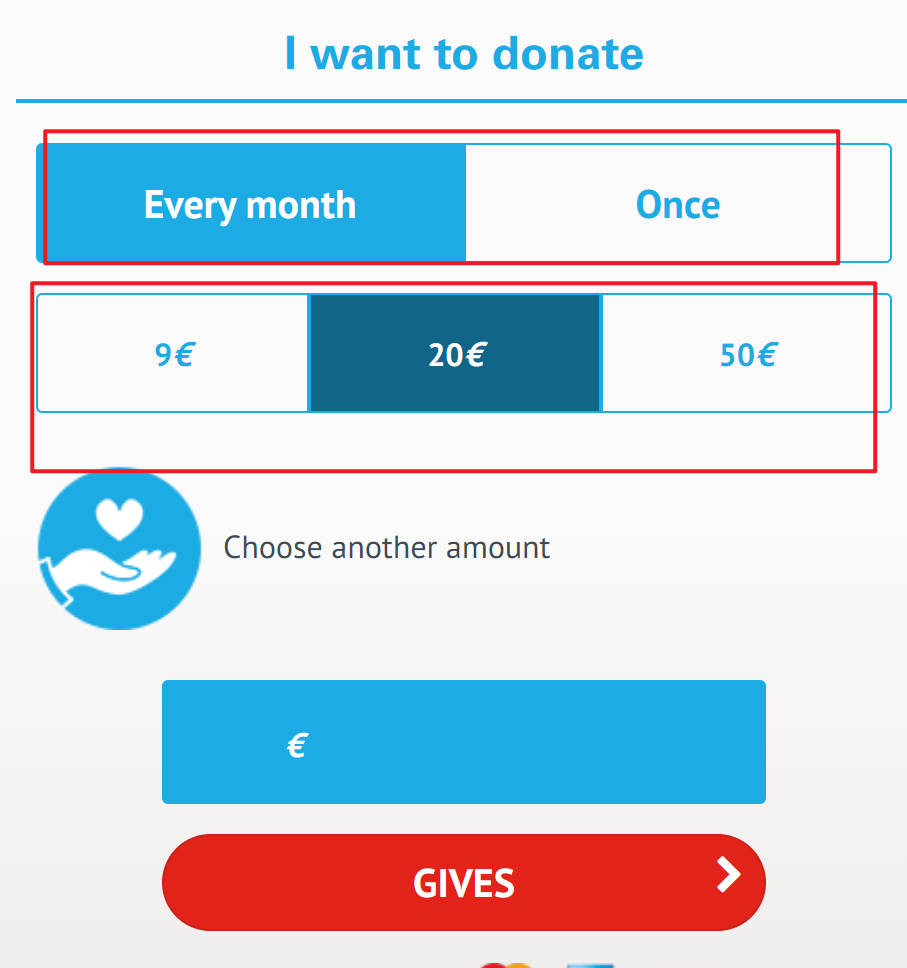
\includegraphics[width=0.5\textwidth]{Resources/Yan/yan_h6.png}
	\caption{Options in the donation page}
	\label{fig:h6}
\end{figure}

\item {\textbf{H7} \color{unicefGray}{Flexibility and efficiency of use}}\\
The website doesn't provide many web accelerators.

\item {\textbf{H8} \color{unicefGray}{Aesthetic and minimalist design}}\\
The website has a user-friendly interface that maintains simplicity and visual elegance.

\item {\textbf{H9} \color{unicefGray}{Help users recognize, diagnose and recover from errors}}\\
The website displays a 404 page if users input the wrong URL. Also, on the donation and sign-in pages, it verifies the valid format of an email
 
\item {\textbf{H10} \color{unicefGray}{Help and documentation}}\\
The website offers all kinds of documents on  https://open.unicef.org/documents. 
\end{description}

\subsubsection{MiLe Heuristics}
\begin{description}
\item {\textbf{M1} \color{unicefGray}{Interaction consistency}}\\
Pages of the same type have the same links and interaction capability.

\item {\textbf{M2} \color{unicefGray}{Group navigation}}\\
Overall, navigating from groups of item lists to their individual members is easy. However, on some pages, it is not possible to return to the previous one.

\item {\textbf{M3} \color{unicefGray}{Navigation support}}\\
The overall Structural navigation is good, but in some places we cannot return to the previous page.

\item {\textbf{M4} \color{unicefGray}{User control}}\\
The website did a great job on semantic navigation. It's quite easy to navigate from one topic to a related one and it also works in the opposite direction.

\item {\textbf{M5} \color{unicefGray}{Error prevention}}\\
“Landmarks”, including header and footer, are useful to reach the key parts of the web site. However, there is still room for the improvement.

\item {\textbf{M6} \color{unicefGray}{Information overload}}\\
 Contents in the organization are massive, but the website find a way to keep the balance, like well-organized menus and precise sentences with dedicate pictures.

\item {\textbf{M7} \color{unicefGray}{Text layout}}\\
The website excels in text layout and offers two distinct designs for different devices, such as PCs and mobile platforms. Texts on various platforms are readable and clear.

\item {\textbf{M8} \color{unicefGray}{Interaction placeholder semiotics}}\\
Icons in the website convey the functional meaning well, E.g.,  A magnifying glass icon for search. And others like icons of reading, research and emergency are intuitive.
\begin{figure}[H]
	\centering
	
\includegraphics[width=0.5\textwidth]{Resources/Yan/yan_m8.png}
	\caption{M8 examples}
	\label{fig:m8}
\end{figure}

\item {\textbf{M9} \color{unicefGray}{Interaction placeholder consistency}}\\
Most textual and labels are consistent.

\item {\textbf{M10} \color{unicefGray}{Spatial allocation}}\\
Overall, the content is well-organized. The on-screen allocation of contents and visuals are appropriate for their relevance. The “semantically related” elements are close and “semantically distant” element are far away.

\item {\textbf{M11} \color{unicefGray}{Consistency of the page structure}}\\
Same type pages follow the same layout(e.g., same visuals and similar layouts).

\item {\textbf{M12} \color{unicefGray}{Coherence in page layout}}\\
Elements on the website are organized in a logical, consistent, and aesthetically pleasing manner, creating a unified and cohesive visual experience for the users.
\end{description}
 	 



